\documentclass[11pt]{ctexrep}
\usepackage{amsmath,amssymb,mathtools,amsthm} % 数学相关宏包
\usepackage{geometry,hyperref}                % 页面布局+超链接
\usepackage{graphicx}                         % 插图宏包
\usepackage{tcolorbox}                         % 定理框宏包
\usepackage{minted}                          % 代码高亮宏包
\usepackage{subcaption}
\usepackage{float}
\tcbuselibrary{theorems,skins}

%% 页面设置
\geometry{margin=1in}
\setlength{\textfloatsep}{10pt plus 2pt minus 2pt}
\renewcommand\thesection{\arabic{section}}
\hypersetup{colorlinks=true,linkcolor=blue,anchorcolor=blue,citecolor=blue}

%% tcolorbox样式（仅用于核心定义/模型，保持原样式）
\tcbset{
    mystyle/.style={
        colback=blue!5,colframe=blue!75!black,
        fonttitle=\bfseries,boxrule=0.8pt,
        left=10pt,right=10pt,top=8pt,bottom=8pt
    }
}
%% 带编号的定义环境（tcolorbox版）
\newtcbtheorem[number within=section]{defn}{定义}{mystyle}{def}
% 普通定理/备注环境
\newtheorem{remark}{注}[section]

%% 标题与作者
\title{BRS Example\\(Dubins' Car)}
\author{武 朝康}
\date{\today}

%% 正文
\begin{document}
\maketitle
%\tableofcontents
\section{引言}
本文以Dubins' Car模型为例，展示如何对其分析，并利用\href{https://github.com/HJReachability/helperOC}{helper\_OC}
工具箱计算其Backward Reachable Set (BRS)。 

Dubins' Car是经典的非线性运动学系统，广泛应用于路径规划与控制问题。本文按照如下步骤展开：
\begin{enumerate}
    \item 定义Dubins' Car的动力学模型与目标集设定。
    \item 构建并分析Hamilton-Jacobi方程。
    \item 利用helper\_OC工具箱计算BRS，并展示结果。
 \end{enumerate}

\section{Dubins' Car模型}
\subsection{动力学模型设定}
在几何学中，术语Dubins path通常指连接二维欧几里得平面（即x-y平面）中两点的最短曲线，该
曲线对路径曲率有约束，路径有规定的初始和终点切线，并且假设形式路径的车辆只能向前行驶。
Dubins path常用于机器人学和控制理论领域，用于规划轮式机器人、飞机和水下航行器的路径。有简单
的几何方法和分析方法可以用于计算最优路径。

例如，在有轮机器人中，一个简单的系统动力学模型（也被称为Dubins' Car）可以表示为：

\begin{equation}
\begin{aligned}
\dot{x} &= v \cos(\theta) \\
\dot{y} &= v \sin(\theta) \\
\dot{\theta} &= u
\end{aligned}
\end{equation}

其中，$(x, y)$ 表示车辆在平面上的位置，$\theta$ 表示车辆的朝向，$v$ 是车辆的速度（通常为常数），
$u$ 是控制输入，代表转向角速度。车辆只能向前行驶，因此 $v > 0$。

为刻画现实中的不确定性，我们引入扰动 $\mathbf{d} = [d_x,d_y,d_{\theta}]^\top$，
定义 $\mathbf{x} = [x,y,\theta]$，则系统动力学可以表示为：
\begin{equation}
\begin{aligned}
\dot{x} &= v \cos(\theta) + d_x \\
\dot{y} &= v \sin(\theta) + d_y \\
\dot{\theta} &= u + d_{\theta}
\end{aligned}
\end{equation}

以上方程可以简洁地写成矩阵形式：%\ref{fig:target_set}：

\begin{equation}
\begin{bmatrix}
\dot{x} \\
\dot{y} \\
\dot{\theta}
\end{bmatrix}
=
\begin{bmatrix}
v \cos(\theta) \\
v \sin(\theta) \\
0
\end{bmatrix}
\,+\,
\begin{bmatrix}
d_x \\
d_y \\
d_{\theta}
\end{bmatrix}
\,+\,
\begin{bmatrix}0 \\ 0 \\ u \end{bmatrix}
\end{equation}

更简洁地，我们可以定义系统的动力学函数 $\mathbf{f}(\mathbf{x},\mathbf{u},\mathbf{d})$，使得系统动力学可以表示为：
\begin{equation}
    \dot{\mathbf{x}} = \mathbf{f}(\mathbf{x},u,\mathbf{d})
\end{equation}

其中，$\mathbf{x}$ 为系统状态，$\mathbf{u} = [0,0,u]^\top$ 为控制输入，$\mathbf{d}$ 为系统扰动。
$\mathbf{u} \in [\mathbf{u}_{\min}, \mathbf{u}_{\max}]$，$\mathbf{d} \in [\mathbf{d}_{\min}, \mathbf{d}_{\max}]$，其中 $\mathbf{u}_{\min}$ 和 $\mathbf{u}_{\max}$ 分别是控制输入的最小值和最大值，$\mathbf{d}_{\min}$ 和 $\mathbf{d}_{\max}$ 分别是系统扰动的最小值和最大值。

\subsection{目标集设定}
接下来定义目标集，即系统期望到达的状态集合：

定义$\theta$的范围为 $[-\pi, \pi]$，二维空间 $x,y$ 的范围为半径为1的一个圆，如下图所示：
\begin{figure}[htbp]
    \centering
    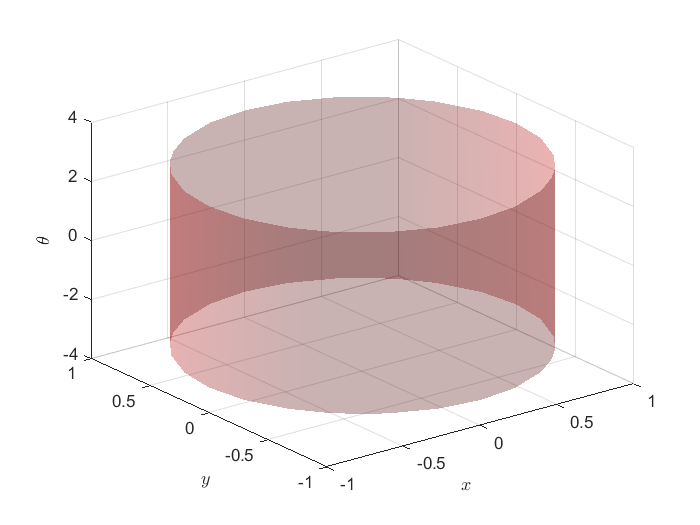
\includegraphics[width=0.5\textwidth]{figures/targetSet.png}
    \caption{目标集示意图}
    \label{fig:target_set}
\end{figure}

处于该区域的状态集合定义为目标集 $\mathcal{T}$。
\section{Hamilton-Jacobi方程分析}
\subsection{问题定义澄清：BRS 与 BRT}
为避免术语混淆，本文统一采用如下约定：
\begin{defn}{BRS 与 BRT 的区别}{brsbrt}
设目标集为 $\mathcal{T}$，时间从负时刻回溯至终端时刻 $0$。
\begin{itemize}
    \item 后向可达集（BRS）：只关注终端时刻是否进入目标集，即要求系统在 $t=0$ 时刻到达 $\mathcal{T}$。
    \item 后向可达管道（BRT）：关注整个时间区间内是否曾进入目标集，即只要在 $[t,0]$ 内某一时刻进入 $\mathcal{T}$ 即可。
\end{itemize}
在 helper\_OC 中，常用 \mintinline{matlab}|'none'| 计算 BRS，\mintinline{matlab}|'minVOverTime'| 计算 BRT。
\end{defn}

\subsection{值函数与 HJ 方程}
后向可达集（Backward Reachable Tube, BRT）定义为集合 $\mathcal{R}(t)$。其表示为
在剩余时间 $t$ 内系统能够从状态 $\mathbf{x}$ 出发，无论受到何种程度的扰动$\mathbf{d}(\cdot)$，
总存在控制策略 $\mathbf{u}(\cdot)$ 使得系统可以在时间间隔 $[t,0]$ 内的某个时刻进入目标集 $\mathcal{T}$ 的状态集合。


针对这个博弈性质的问题，定义值函数（Value Function）为：
\begin{equation}
\begin{aligned}
V(\mathbf{x},t)
= \inf_{\mathbf{u}(\cdot)} \sup_{\mathbf{d}(\cdot)}
\min_{\tau \in[t,0]} \ell\!\left(\mathbf{x}_{\mathbf{x},t}^{\mathbf{u},\mathbf{d}}(\tau)\right)
\end{aligned}
\end{equation}

其中，$\mathbf{x}(\tau)$ 表示系统在控制与扰动共同作用下、由时刻 $t$ 的状态 $\mathbf{x}$ 出发的演化轨迹。
公式内的$\min_{\tau}$ 体现了“管道（Tube）”的概念，即只要轨迹在演化过程中的任意瞬间进入目标集，该初始
状态即属于可达集。


最终，后向可达集可以表示为值函数的零水平集：
\begin{equation}
\mathcal{R}(t) = \{\mathbf{x} \in \mathbb{R}^n \mid V(\mathbf{x},t) \leq 0\}
\end{equation}

值得注意的是，当 $t=0$ 时，根据定义可知 $V(\mathbf{x},0) = \ell(\mathbf{x})$，即
此刻的后向可达集等于目标集 $\mathcal{T}$。随着时间向过去回溯，$\mathcal{R}(t)$ 随之演化。
为了求解该值函数的变化，需要求解如下Hamilton-Jacobi偏微分方程：
\begin{equation}
\frac{\partial V}{\partial t} + \min \left(
0,\ \ 
\min_{\mathbf{u} \in \mathcal{U}} \max_{\mathbf{d} \in \mathcal{D}} \nabla V ^\top \cdot \mathbf{f}(\mathbf{x},\mathbf{u},\mathbf{d})
\right)
 = 0
\end{equation}

式中，$\nabla V$ 表示值函数 $V$ 关于状态 $\mathbf{x}$ 的梯度，即
$\nabla V = [\partial V / \partial x, \partial V / \partial y, \partial V / \partial \theta]^\top$，
$\mathbf{f}(\mathbf{x},\mathbf{u},\mathbf{d})$ 是系统的动力学函数。


定义Hamiltonian：
\begin{equation}
H^* = \min_{\mathbf{u} \in \mathcal{U}} \max_{\mathbf{d} \in \mathcal{D}} \nabla V \cdot \mathbf{f}(\mathbf{x},\mathbf{u},\mathbf{d})
\end{equation}

将$\nabla V$记为$[p_x, p_y, p_{\theta}]^\top$，则Hamiltonian可以写为：
\begin{equation}
\begin{aligned}
    H^* &= \min_{\mathbf{u}}\max_{\mathbf{d}} \left( p_x \dot{x} + p_y \dot{y} +p_{\theta} \dot{\theta} \right)\\
    &= \min_{\mathbf{u}}\max_{\mathbf{d}} \left( p_x (v \cos(\theta) + d_x) + p_y (v \sin(\theta) + d_y) +p_{\theta} (u + d_{\theta}) \right)\\
    &= p_x v \cos(\theta) + p_y v \sin(\theta)
    + \min_{\mathbf{u}} (p_{\theta} u)
    + \max_{\mathbf{d}} (p_x d_x + p_y d_y + p_{\theta} d_{\theta})
\end{aligned}
\end{equation}

因此，Hamiltonian的最优控制输入 $\mathbf{u}^*$ 和最优扰动 $\mathbf{d}^*$ 可以通过以下优化问题求解：
\begin{equation}
\begin{aligned}
\mathbf{u}^* &= \arg\min_{\mathbf{u} \in \mathcal{U}} (p_{\theta} u) 
\end{aligned}
\end{equation}

当 $p_{\theta} \ge 0$ 时， 最优控制输入 $\mathbf{u}^* = u_{\min}$；当 $p_{\theta} < 0$ 时，最优控制输入 $\mathbf{u}^* = u_{\max}$；当 $p_{\theta} = 0$ 时，最优控制输入 $\mathbf{u}^*$ 可以取任意值。


\begin{equation}
\begin{aligned}
d_x^* &= \arg\max_{d_x} (p_x d_x) \\
d_y^* &= \arg\max_{d_y} (p_y d_y) \\
d_{\theta}^* &= \arg\max_{d_{\theta}} (p_{\theta} d_{\theta})
\end{aligned}
\end{equation}

对任意分量 $i \in \{x,y,\theta\}$，当 $p_i \ge 0$ 时，最优扰动 $d_i^* = d_{i,\max}$；当 $p_i < 0$ 时，最优扰动 $d_i^* = d_{i,\min}$；当 $p_i = 0$ 时，最优扰动 $d_i^*$ 可以取任意值。

上述结果给出了最优控制与最优扰动的解析选取方式，并可直接用于控制系统实现。若控制空间更复杂或输入不满足仿射结构，
可采用数值优化求解器获得对应的最优策略。

另外，如果我们定义的后向可达集是终端时间到达，也就是系统在时间 $t=0$ 时必须进入目标集 $\mathcal{T}$，
其余时间进入均不算，则Hamilton-Jacobi方程中的最小值项可以省略：
\begin{equation}
\frac{\partial V}{\partial t} + \min_{\mathbf{u} \in \mathcal{U}} \max_{\mathbf{d} \in \mathcal{D}} \nabla V ^\top \cdot \mathbf{f}(\mathbf{x},\mathbf{u},\mathbf{d})
 = 0    
\end{equation}


\section{数值求解与结果展示}
\subsection{数值求解设置}
为了求解上述Hamilton-Jacobi方程，使用helper\_OC工具箱进行数值计算。该工具箱定义了一套函数接口，允许用户
定义动力学系统，优化控制选取和扰动选取，并求解Hamilton-Jacobi方程以获得后向可达集。
Dubins' Car 的动力学模型在本工具箱中已有定义，直接使用即可。

首先定义系统状态空间。

\begin{minted}[frame=single, framesep=10pt]{matlab}
%% 1. 网格定义
grid_min = [-5; -5; -pi];    % 计算区域的下边界
grid_max = [5; 5; pi];       % 计算区域的上边界
N = [41; 41; 41];            % 每一个维度的网格点数目
pdDims = 3;                  % 第三个维度是周期性
g = createGrid(grid_min, grid_max, N, pdDims);
% 使用 "g = createGrid(grid_min, grid_max, N);" 如果不存在周期性维度
\end{minted}

进一步的，我们定义目标集 $\mathcal{T}$：

\begin{minted}[frame=single, framesep=10pt]{matlab}
R = 1;
data0 = shapeCylinder(g, 3, [0; 0; 0], R);
% 可以尝试其他的目标集形状 shapeRectangleByCorners, shapeSphere.
\end{minted}

时间向量定义：
\begin{minted}[frame=single, framesep=10pt]{matlab}
%% 时间向量
t0 = 0;
tMax = 2;
dt = 0.05;
tau = t0:dt:tMax;
\end{minted}

定义动力学系统的参数：
\begin{minted}[frame=single, framesep=10pt]{matlab}
%% 问题参数
speed = 1;      % 车辆的速度（常数）
% 输入边界·扰动定义
wMax = 1;
dMax = [.25, .25, 0];
% 存在控制·任意扰动
uMode = 'min';
dMode = 'max';    
dCar = DubinsCar([0, 0, 0], wMax, speed, dMax); % 生成DubinsCar动力学系统
% dCar = DubinsCar([0, 0, 0], wMax, speed); % (没有扰动版)
\end{minted}  

打包问题参数进入求解器：
\begin{minted}[frame=single, framesep=10pt]{matlab}
%% 将问题参数打包进 schemeData
% 将网格和动力学系统打包进 schemeData
schemeData.grid = g;
schemeData.dynSys = dCar;
schemeData.accuracy = 'high'; % 设置求解精度 
schemeData.uMode = uMode;
schemeData.dMode = dMode;
\end{minted}


下面给出值函数演化的求解过程：
\begin{minted}[frame=single, framesep=10pt]{matlab}
HJIextraArgs.visualize.valueSet = 1;
HJIextraArgs.visualize.initialValueSet = 1;
HJIextraArgs.visualize.figNum = 1; % 设置图像编号
HJIextraArgs.visualize.deleteLastPlot = true; % 删除上一次的图像
HJIextraArgs.visualize.plotData.plotDims = [1 1 0]; % 画 x, y
HJIextraArgs.visualize.plotData.projpt = [0]; % 投影 theta = 0
HJIextraArgs.visualize.viewAngle = [0,90]; % 可视化角度（俯视图）
[data, tau2, ~] = ...
  HJIPDE_solve(data0, tau, schemeData, 'minVOverTime', HJIextraArgs);
\end{minted}

经过求解，我们已经得到了值函数 $V(\mathbf{x},t)$ 在不同时刻的数值解 \mintinline{matlab}|data| 。
据此，我们可以求解出任意时刻的后向可达集 $\mathcal{R}(t)$，即值函数的零水平集。以 $t=-2$ 为例（注意其对应的是 $tau = 2$）：
\begin{minted}[frame=single, framesep=10pt]{matlab}
    figure();    h = visSetIm(g, data(:,:,:,end)); 
    h.alpha = 0.3;      grid on; % 设置透明度
\end{minted}
\subsection{结果展示与对比}
通过上述代码，我们可以可视化后向可达集在三维空间中的形状，如图 \ref{fig:brt_disturbance_3d} 所示。根据定义，
处于该集合内的状态 $\mathbf{x}$ 可以在时间 $t=-2$ 内通过适当的控制输入 $u$ 和任意扰动 $d$ 的作用下进入目标集 $\mathcal{T}$。
\begin{figure}[htbp]
    \centering
    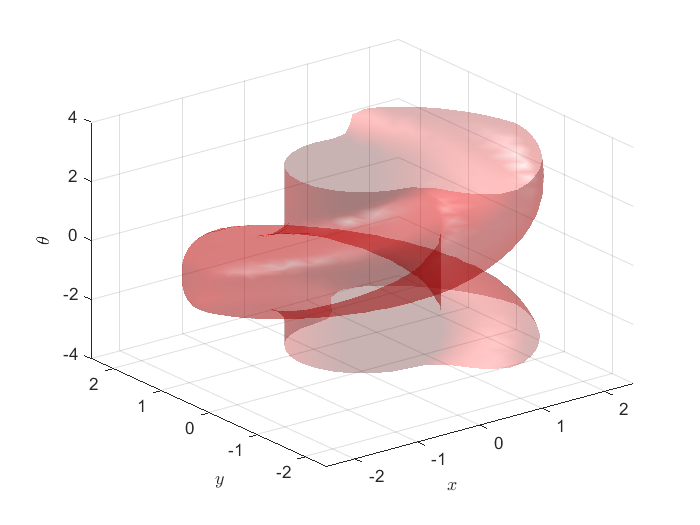
\includegraphics[width=0.5\textwidth]{figures/BRT(disturbance).png}
    \caption{后向可达集（有扰动）}
    \label{fig:brt_disturbance_3d}
\end{figure}

假设一初始状态点为 $x_{\text{init}} = [2, 0, \pi]$，由目标集的半径 $R = 1$ 可以得知，该点在目标集之外。
下面我们观察其在 $-2 \rightarrow 0$ 的演化轨迹。 

\begin{minted}[frame=single, framesep=10pt]{matlab}
    xinit = [2; 0; pi];
    value = eval_u(g, data(:,:,:,end), xinit); % 计算初始状态点的值函数值
    if value <=0
        dCar.x = xinit;
        TrajextraArgs.uMode = uMode;    % 设置控制模式
        TrajextraArgs.dMode = 'max';    % 设置扰动模式
        TrajextraArgs.visualize = true; % 可视化
        TrajextraArgs.fig_num = 2;      % 图像编号
        TrajextraArgs.projDim = [1 1 0]; % 投影维度
        % 翻转数据时间点，使我们从时间的开始点开始计算轨迹
        dataTraj = flip(data, 4);
        [traj, traj_tau] = ...
        computeOptTraj(g, dataTraj, tau2, dCar, TrajextraArgs);
    else     
        error(['初始状态不在 BRS/BRT 中! 其value为 ' num2str(value,2)])
    end
\end{minted}

代码中的 \mintinline{matlab}|computeOptTraj| 函数用于计算从初始状态点 $x_{\text{init}}$ 出发的最优轨迹，
该轨迹在时间 $t=-2$ 到 $t=0$ 的过程中，受到最优控制输入 $u^*$ 和最优扰动 $d^*$ 的作用。最终的轨迹结果如图 \ref{fig:trajectory} 所示。

\begin{figure}[htbp]
    \centering
    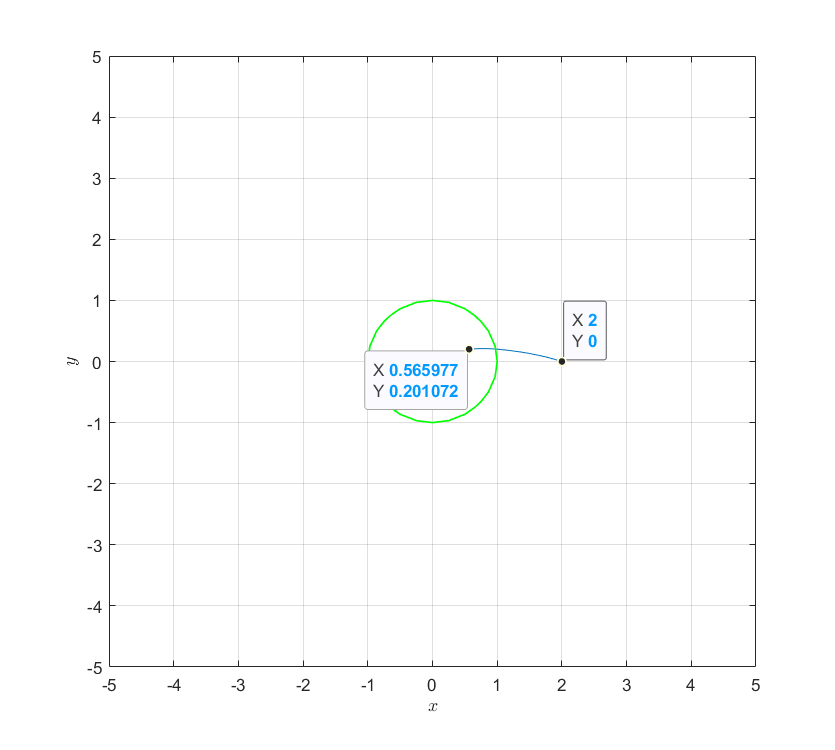
\includegraphics[width=0.5\textwidth]{figures/traj&targetSet.png}
    \caption{演化轨迹与目标集}
    \label{fig:trajectory}
\end{figure}

图 \ref{fig:trajectory} 中，蓝色曲线代表状态点从初始位置 $x_{\text{init}}$ 出发的演化轨迹，
绿色圆圈表示目标集 $\mathcal{T}$ 的边界。可以观察到，该状态最终进入了目标集。


进一步考察无扰动情形，即 $\mathbf{d} = \mathbf{0}$ 时后向可达集 $\mathcal{R}(t)$ 的变化，结果如下：

\begin{figure}[H]
    \centering
    % disturbance 子图
    \begin{subfigure}[t]{0.4\textwidth}
        \centering
        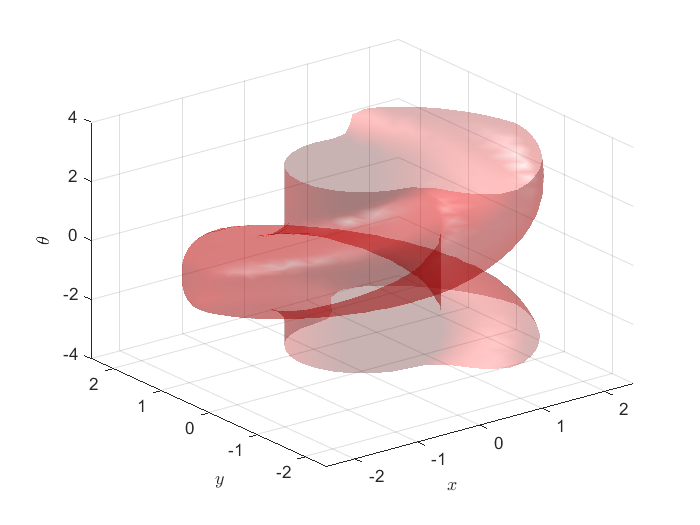
\includegraphics[width=\textwidth]{figures/BRT(disturbance).png}
        \caption{后向可达集（有扰动）}
        \label{fig:brt_disturbance_compare}
    \end{subfigure}\hspace{0.05\textwidth}%
    % no disturbance 子图
    \begin{subfigure}[t]{0.4\textwidth}
        \centering
        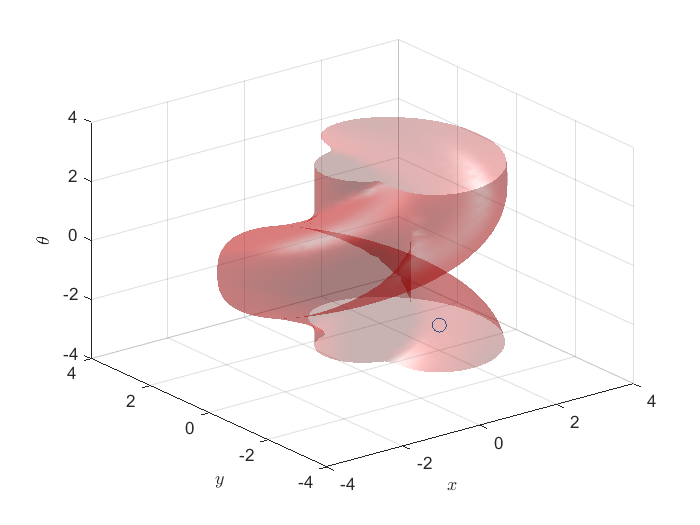
\includegraphics[width=\textwidth]{figures/BRT(no disturbance).png}
        \caption{后向可达集（无扰动）}
        \label{fig:brt_no_disturbance_compare}
    \end{subfigure}
    \caption{后向可达集对比：(a) 有扰动；(b) 无扰动}
    \label{fig:brt_compare}
\end{figure}

为更直观地比较平面位置分量，给出俯视图如下：
\begin{figure}[H]
    \centering
    % disturbance 子图
    \begin{subfigure}[t]{0.4\textwidth}
        \centering
        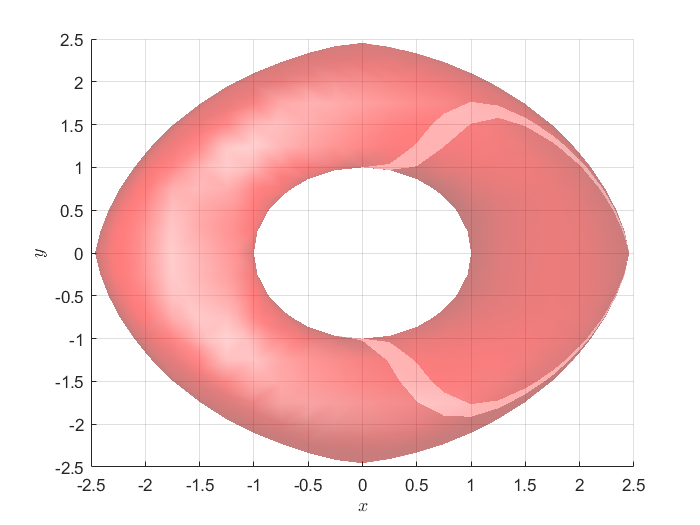
\includegraphics[width=\textwidth]{figures/BRT(disturbance u-d).png}
        \caption{后向可达集（有扰动，俯视）}
        \label{fig:brt_disturbance_top}
    \end{subfigure}%
    \hspace{0.05\textwidth}%
    % no disturbance 子图
    \begin{subfigure}[t]{0.4\textwidth}
        \centering
        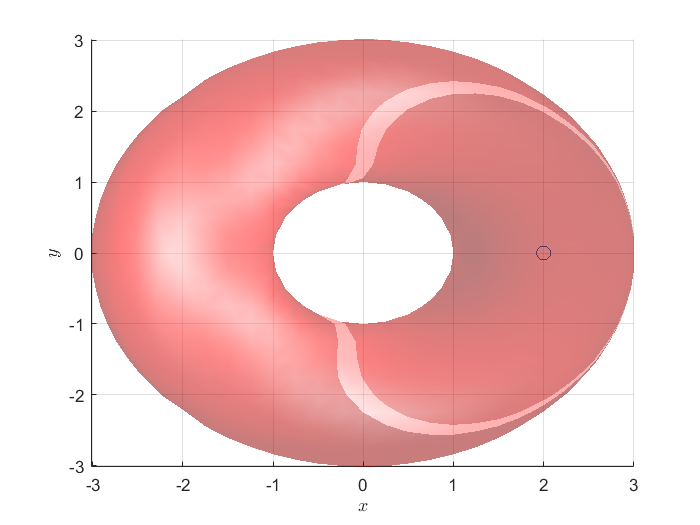
\includegraphics[width=\textwidth]{figures/BRT(no disturbance u-d).png}
        \caption{后向可达集（无扰动，俯视）}
        \label{fig:brt_no_disturbance_top}
    \end{subfigure} 
    \caption{俯视后向可达集对比：(a) 有扰动；(b) 无扰动}
    \label{fig:brt_top_compare}
\end{figure}

结果表明，无扰动条件下后向可达集 $\mathcal{R}(t)$ 的范围显著增大。这是因为存在扰动时系统需对最坏情形进行鲁棒考虑，
其可达区域因而受到更强约束。

进一步，我们观察值函数（value function）的变化。如下图所示：

\begin{figure}[htbp]
    \centering
    \begin{subfigure}[t]{0.3\textwidth}
        \centering
        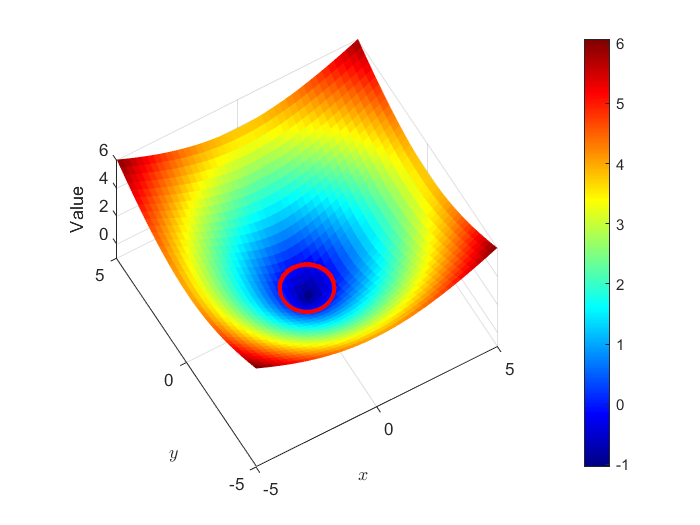
\includegraphics[width=\textwidth]{figures/valFuc(no disturbance)0.png}
        \caption{0时刻的值函数（无扰动）}
        \label{fig:val_no_disturbance_t0}
    \end{subfigure}
    \hfill
    \begin{subfigure}[t]{0.3\textwidth}
        \centering
        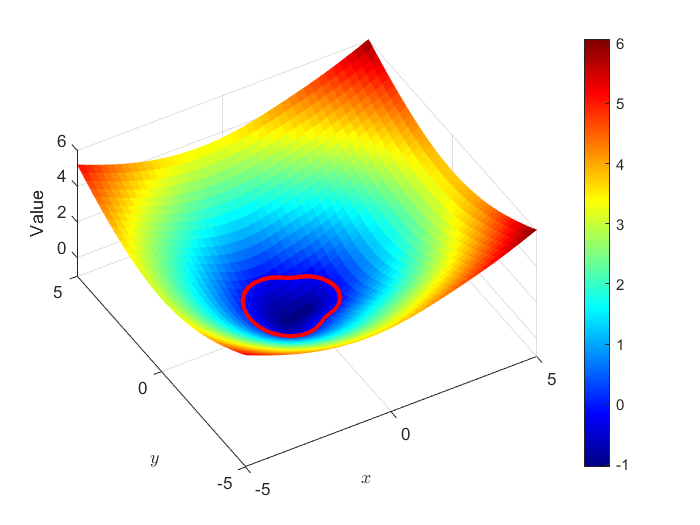
\includegraphics[width=\textwidth]{figures/valFuc(no disturbance)-1.png}
        \caption{-1时刻的值函数（无扰动）}
        \label{fig:val_no_disturbance_t1}
    \end{subfigure} 
    \hfill
    \begin{subfigure}[t]{0.3\textwidth}
        \centering
        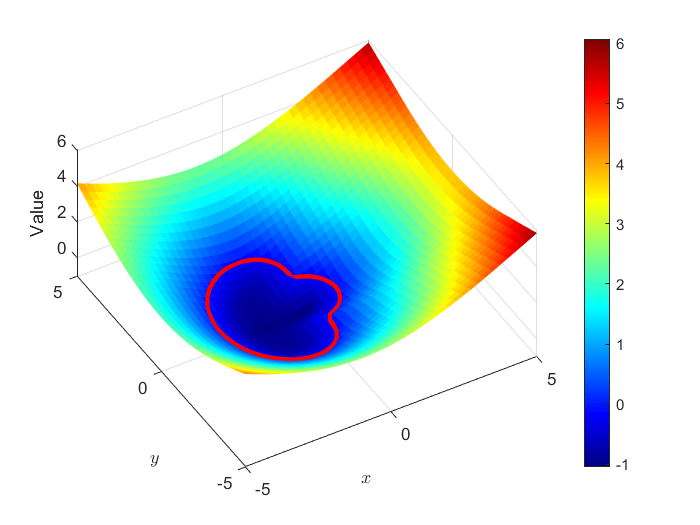
\includegraphics[width=\textwidth]{figures/valFuc(no disturbance)-2.png}
        \caption{-2时刻的值函数（无扰动）}
        \label{fig:val_no_disturbance_t2}
    \end{subfigure}
    \caption{无扰动值函数演变(a) 0时刻；(b) -1时刻；(c) -2时刻}
    \label{fig:val_no_disturbance_evolution} 
\end{figure}

图中红色曲线内部区域对应值函数为负的区域，即后向可达集 $\mathcal{R}(t)$。可以观察到：
\begin{enumerate}
\item 0时刻的可达集区域最小，仅包含目标集 $\mathcal{T}$。
\item 随着时间向过去回溯，值函数为负的区域变大，可达集区域扩大，包含了更多的状态。
\item 0时刻的可达集区域在后续时刻被包含在更大的可达集区域内。
\end{enumerate}

需要指出的是，当计算对象为后向可达集（而非后向可达管道）时，第2条结论一般不成立。

此处不再展示轨迹与三维可达集，仅从值函数演化角度进行说明。
这需要我们调用 \mintinline{matlab}|HJIPDE_solve| 函数，将参数 \mintinline{matlab}|minWith| 设置为 \mintinline{matlab}|'none'|。
\begin{minted}[frame=single, framesep=10pt]{matlab}
[data, tau, ~] = ...
  HJIPDE_solve(data0, tau, schemeData, 'none', HJIextraArgs);
\end{minted}

其值函数（value function）的演变如下图所示：

\begin{figure}[htbp]
    \centering
    \begin{subfigure}[t]{0.3\textwidth}
        \centering
        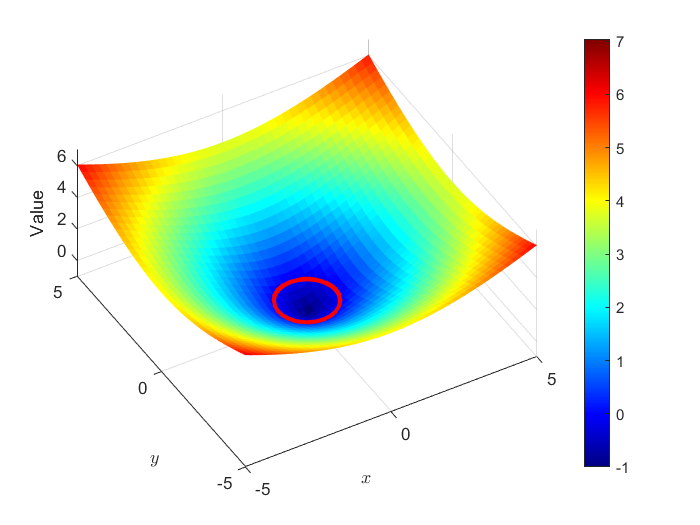
\includegraphics[width=\textwidth]{figures/valFuc(BRS no disturbance)0.png}
        \caption{0时刻的值函数（无扰动）}
        \label{fig:val_brs_no_disturbance_t0}
    \end{subfigure}
    \hfill
    \begin{subfigure}[t]{0.3\textwidth}
        \centering
        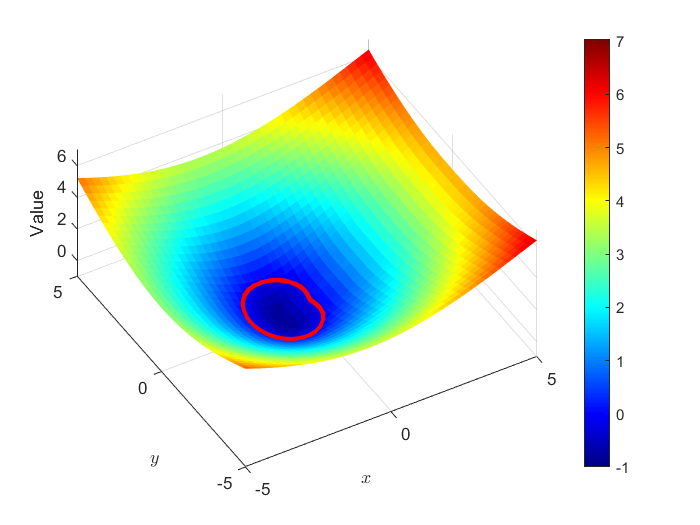
\includegraphics[width=\textwidth]{figures/valFuc(BRS no disturbance)-1.png}
        \caption{-1时刻的值函数（无扰动）}
        \label{fig:val_brs_no_disturbance_t1}
    \end{subfigure} 
    \hfill
    \begin{subfigure}[t]{0.3\textwidth}
        \centering
        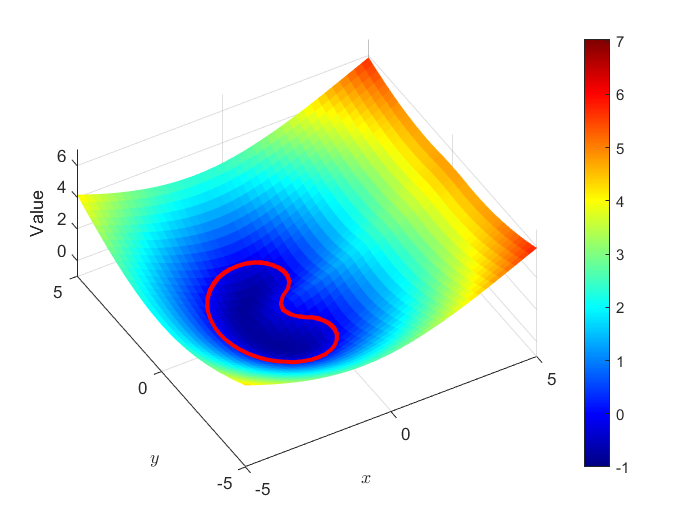
\includegraphics[width=\textwidth]{figures/valFuc(BRS no disturbance)-2.png}
        \caption{-2时刻的值函数（无扰动）}
        \label{fig:val_brs_no_disturbance_t2}
    \end{subfigure}
    \caption{无扰动BRS值函数演变(a) 0时刻；(b) -1时刻；(c) -2时刻}
    \label{fig:val_brs_no_disturbance_evolution} 
\end{figure}

可以看出，在无扰动条件下，值函数负区域（即后向可达集）扩展更快且覆盖更广。同时，0时刻可达区域在后续时刻不一定保持集合包含关系。
这是因为某些状态可在1 s内进入目标集，但在2 s时未必仍满足终端到达约束；而此处BRS仅关注终端时刻（$t=0$）是否进入目标集。

综上，本文完成了Dubins' Car模型下后向可达集问题的建模、方程分析与数值求解。通过有扰动与无扰动情形的对比，可清晰识别扰动对系统可达性的影响及值函数演化规律。
同时，文中对BRS与BRT在定义与结果层面的差异进行了对照说明，为后续在更复杂系统中的可达性分析提供了参考。

\end{document}